\documentclass[a4paper,12pt]{article}
\usepackage[utf8]{inputenc}
\usepackage{geometry}
\usepackage{xcolor}
\usepackage{hyperref}
\usepackage{tcolorbox}
\tcbuselibrary{skins, breakable}
\usepackage{listings}
\usepackage{fancyvrb}
\usepackage{pdfpages}

% 1. Setup the Markdown Package
% This package renders external .md files
\usepackage[
  hybrid,   % Allows standard LaTeX commands inside markdown
  fencedCode,
  smartEllipses,
  pipeTables,
  tableCaptions,
  underscores=false,
  definitionLists,
  inlineFootnotes,
  footnotes,
  hashEnumerators,
  strikeThrough
]{markdown}

% Configure markdown rendering options
\markdownSetup{
  rendererPrototypes={
    headingOne = {\section{#1}},
    headingTwo = {\subsection*{#1}},
    headingThree = {\subsubsection*{#1}},
    horizontalRule = {\vspace{0.5em}\noindent\rule{\textwidth}{0.4pt}\vspace{0.5em}}
  }
}

% Configure code block styling
\lstset{
  basicstyle=\ttfamily\small,
  breaklines=true,
  frame=single,
  backgroundcolor=\color{gray!10},
  xleftmargin=10pt,
  xrightmargin=10pt,
  framexleftmargin=5pt,
  framexrightmargin=5pt,
  numbers=none
}

% 2. Define Visual Styles for the Chat
\newtcolorbox{chatbox}{
  colback=white,      % White background
  colframe=gray!30,    % Light gray border
  fonttitle=\sffamily\bfseries,
  coltitle=black,
  breakable,           % Allows the chat to split across pages
  enhanced,
  boxrule=0.5pt,
  left=15pt, right=15pt, top=10pt, bottom=10pt,
  sharp corners
}

% Configure page geometry for better readability
\geometry{
  left=2.5cm,
  right=2.5cm,
  top=2.5cm,
  bottom=2.5cm
}

\title{AI Appendix - AE4868}
\author{Ismael Gallo López} % Replace with your name
\date{\today}

\begin{document}

\maketitle

Gemini ha dicho
\section*{AI Usage Summary}

\section*{AI Usage Declaration}

\subsection*{Description of Usage}

For this assignment, AI tools were used exclusively for debugging assistance, conceptual verification, plotting architecture, and LaTeX formatting.

Specifically, AI was consulted to:

\begin{itemize}
\item Clarify underlying Tudatpy C++ API structures and resolve argument TypeError crashes.
\item Differentiate between API classes (e.g., step size validation vs. control settings) and debug structural logic in nested simulation loops.
\item Generate Python matplotlib boilerplate code to extract, format, and visualize the numerical propagation data in accordance with the course's AI visualization exception.
\item Conceptually discuss the mathematical behavior of integrators, such as truncation error dominance, Lagrange interpolator boundaries, and the "accuracy floor" of benchmarks.
\item Format specific mathematical notations and cross-referencing commands in LaTeX.
\end{itemize}

AI was not used to blindly generate the core propagation algorithms, solve the differential correctors from scratch, or bypass the fundamental learning objectives. All mathematical formulations, implementation logic, and final physics analyses were developed independently and only refined through discussion.

\section*{Question 1 - AI Usage}

\subsection*{Description of Usage}
AI was used to review the initial script to identify missing assignment requirements (extracting maximum error arrays). It was heavily utilized to generate the Python matplotlib code for plotting the error over time (1a) and maximum error versus step size (1b). Additionally, AI provided LaTeX syntax corrections for rendering discrete mathematical subsets (Δt∈{...}) and reusing footnote references.

\section*{Question 2 - AI Usage}

\subsection*{Description of Usage}
AI acted as a conceptual sounding board to structure the logic for comparing the Δt/2 method and the benchmark method without generating the underlying Tudat execution code. It provided the logical framework for avoiding crashes caused by the 8th-order Lagrange interpolator boundary conditions. Finally, AI generated the plotting scripts for 2a, 2b, and 2c, including suggesting a conceptual shift from plotting the absolute error difference to plotting the relative error ratio for clearer physical analysis.

\section*{Question 3 - AI Usage}

\subsection*{Description of Usage}
AI was consulted to identify a structural logic flaw in the provided skeleton code regarding the placement of variable tolerance settings outside the iteration loop. It generated the plotting scripts for the variable step size error and step-history (3a and 3b), and later adapted them for the blockwise step control requirements (3c and 3d). AI was also used to conceptually discuss methods for accurately computing the GCO500 orbital period from initial state data, and to verify that sharp drops in step sizes were a physically expected behavior of the control algorithm rather than a software bug.

\section*{Question 4 - AI Usage}

\subsection*{Description of Usage}
AI was used for theoretical discussions regarding the "U-curve" of numerical integration and why a rounding-error-dominated setup is mathematically invalid as a benchmark. It generated the complex plotting architecture for the workload diagram (Q4a), estimating function evaluations based on Runge-Kutta stages. Additionally, AI was consulted to explain the "accuracy floor" phenomenon observed when comparing highly precise integrators (10 
−14
  tolerance) against the fixed 10s/20s benchmark assigned for grading coherence.

\section*{Question 5 - AI Usage}

\subsection*{Description of Usage}
AI was used to debug the numerical extraction loop, successfully identifying a variable assignment error that was causing the Euler integrator to take a 300-second step instead of a 10-second step. In accordance with the conceptual discussion guidelines, AI assisted in transcribing and structuring the analytical Taylor series derivations for the theoretical error constants (K 
r
​
 ) for both the RKF7(8) and Euler integrators in circular orbits. Finally, AI provided the plotting code to compare the numerical extractions to these theoretical derivations, including a relative percentage error plot.
\subsection*{General Chat Transcript}

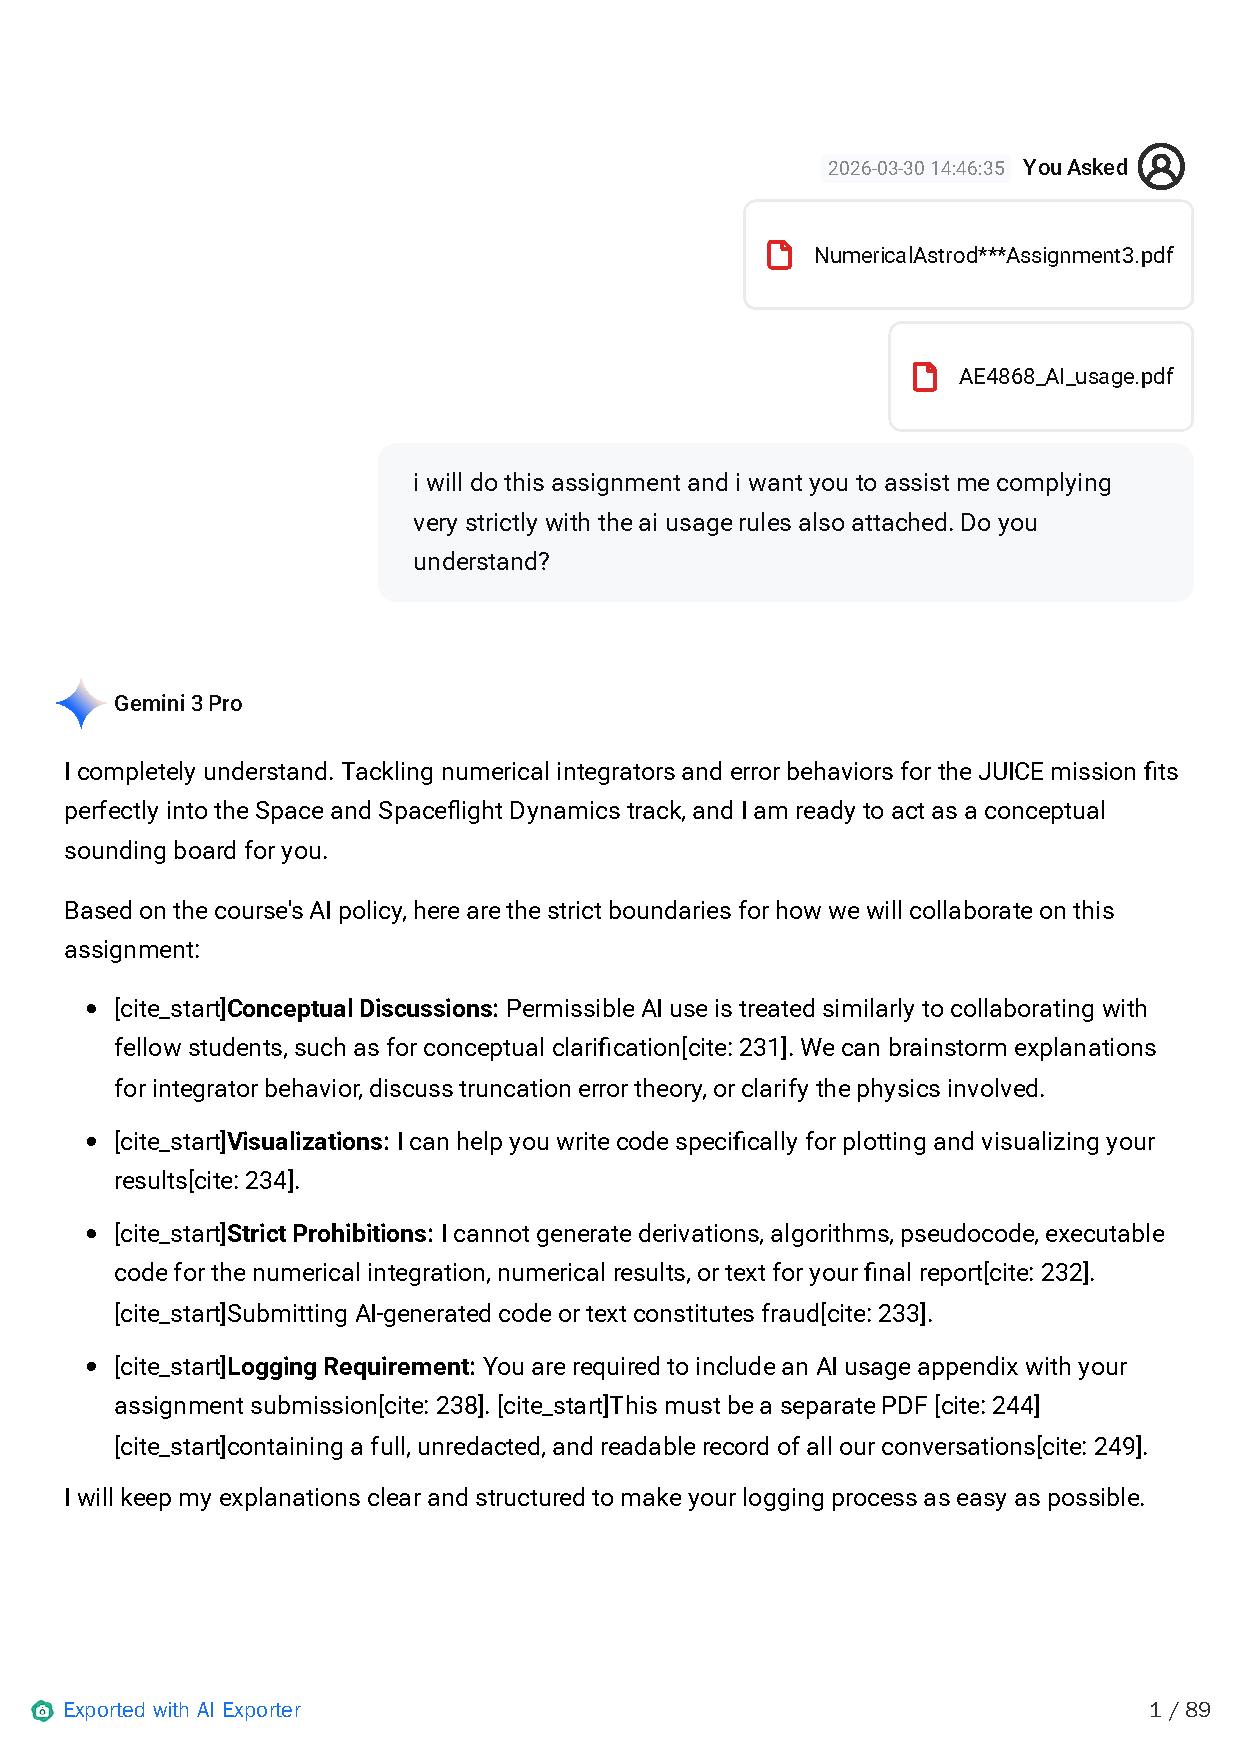
\includepdf[pages=-,pagecommand={},scale=0.95,frame=false]{_NA - Assignment 3 Conversación fijada.pdf}

\end{document}